\section{X-Learning  Architecture}
\label{sec:x-learning_architecture}

A Web application developed by using the x-project toolkit, is a full stack JavaScript Single Page Application.


\subsection{Server side}
\label{subsec:server_side}

On the server side, an X-Learning app is based on NodeJS (see \ref{sec:nodejs}) used to create the server environment, MongoDB (see \ref{sec:mongodb}) used to storage data, and the Web framework Loopback by Strongloop (see \ref{sec:strongloop_loopback}).
Node.js is a JavaScript runtime built on Chrome’s  V8  JavaScript  engne. Node.js uses an event-driven, non-blocking I/O model that makes it lightweight and efficient. Node.js’ package ecosystem, npm, is the largest ecosystem of open source libraries in the world. NodeJS lets to create a vertical full-stack application in Javascript. The NodeJS asynchronous development scheme increases performances of web applications, by using downtime caused  by  HTTP requests.
LoopBack generates model API from the models schemas, to let CRUD operations on models. Loopback is the core of the X-Learning server-side. Document oriented API definition guarantees easiness and speed in API creation. Moreover, Loopback, is fully compatible with several DBMS thanks to connectors.
MongoDB is a cross-platform document-oriented database.  Classified as a NoSQL database, MongoDB eschews the traditional table-based relational database structure in favor of JSON-like documents with dynamic schemas. The document-oriented being of MongoDB allows to horizontal scale in really easy way. Moreover, document models, that replace relational database’s rows, are schemaless: this feature gives to MongoDB project high levels of flexibility and manageability.

\subsection{Client side}
\label{subsec:client_side}

On the client side, an X-Learning app is based on HTML5 Web Components via Polymer-Project by Google. It is a set of Polymer elements for local routing, API request, forms, lists, style and admin panels.
Polymer-Project is one of the most important emerging realities of the moment. Google team has heavily focused his forces on code reusability and on separation between behavior, presentation and content.  Code reusability is a direct effect of Web Components structure: the creation of widget that can be completely indipendent facilitates code reuse.
Finally, the union between Polymer and Strongloop has been topped by the creation of the document oriented development process described below \ref{sec:x-learning_design}.

\begin{figure}[htb] %  figure placement: here, top, bottom
 \centering
 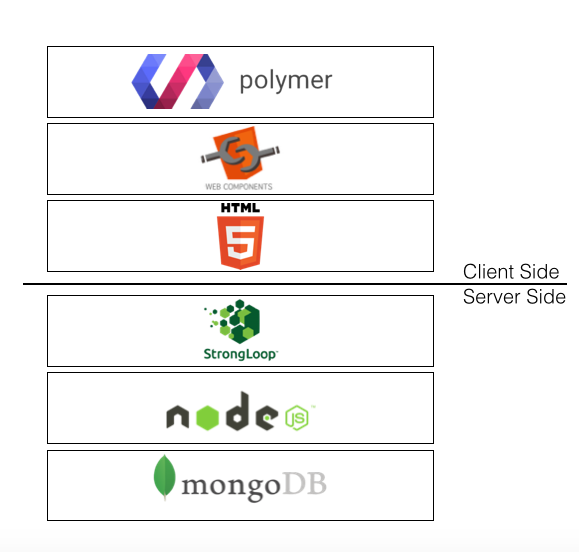
\includegraphics[width=1.0\linewidth]{images/chapter4/XPR_stack.png}\hfill
 \caption[X-learning Architectural Stack]{X-Learning Architectural Stack}
 \label{fig:fourV}
\end{figure}